\chapter{Quasi-spherical collapse}
\label{sec: Sim}

\section{Initial conditions} \label{sec: Sim: IC}

Here's three figures together using minipage

\begin{figure}[th!]
    \centering
    \begin{minipage}{.49\textwidth}
        \centering
        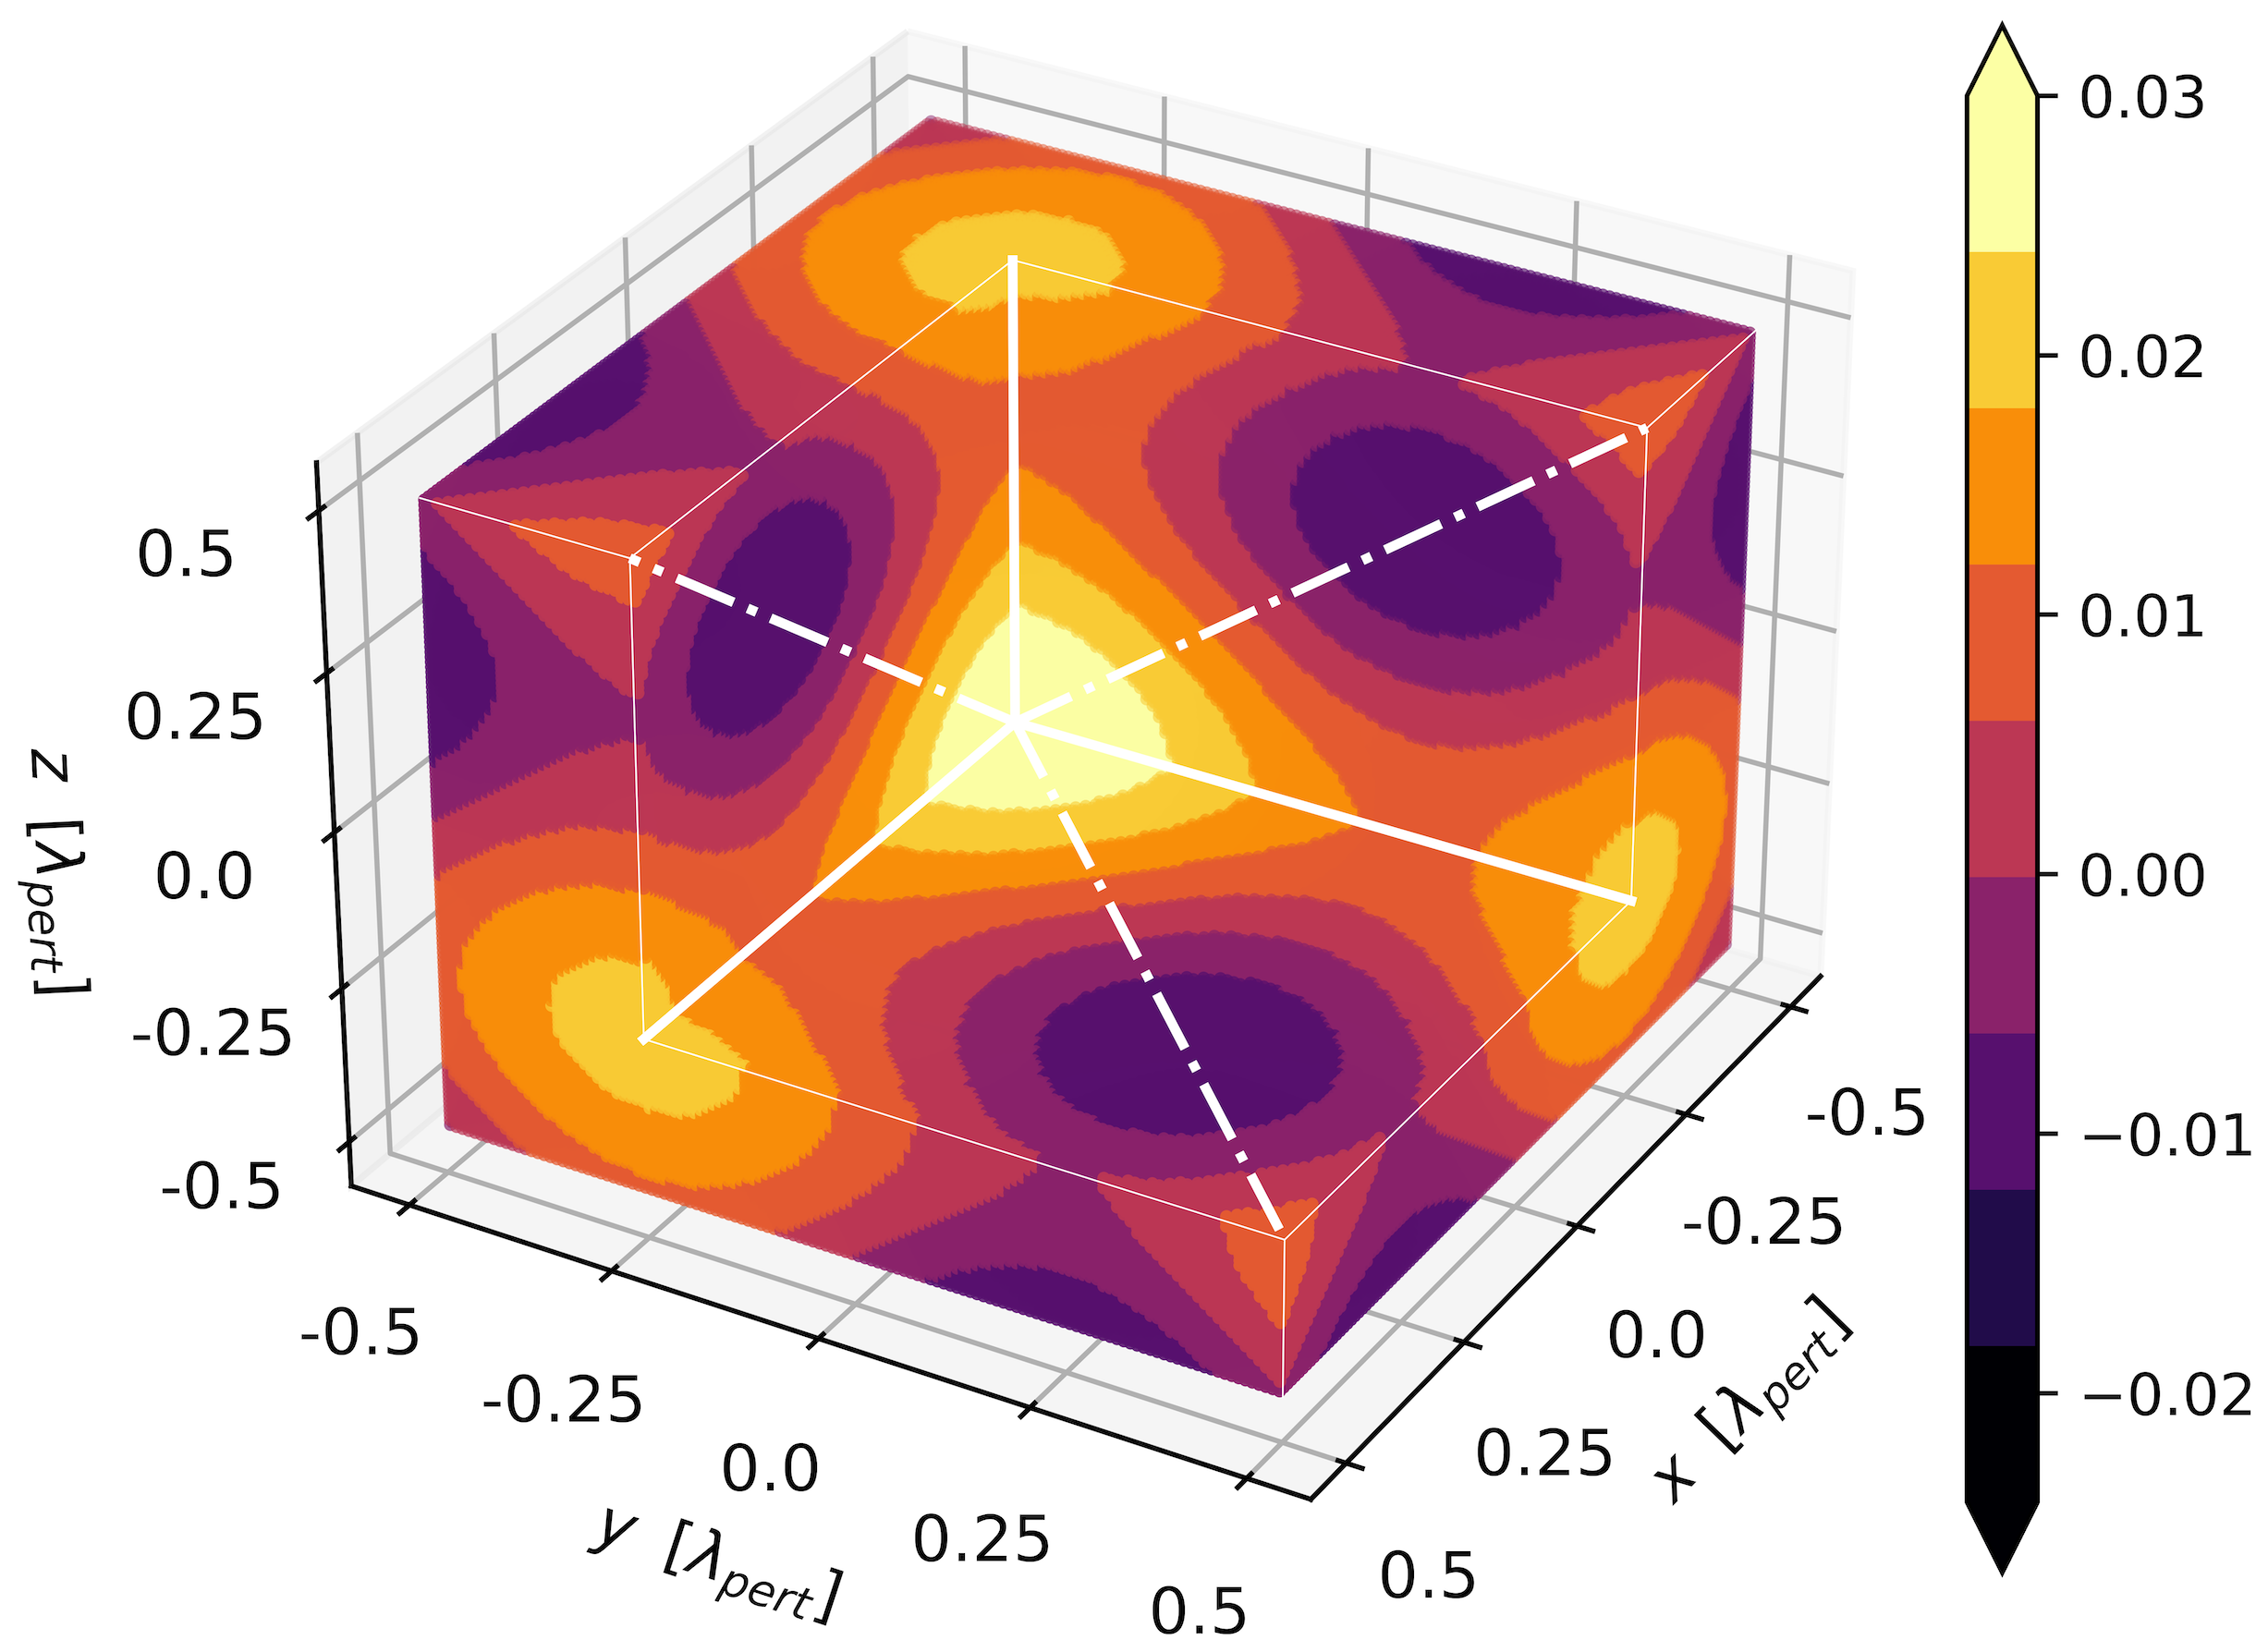
\includegraphics[width=\linewidth]{plots/Paper2/Initial_3d_delta.png}
        \caption[Initial $\delta$ in the simulation box]{Initial distribution at $z_{IN} = 302.5$ of the density contrast $\delta$ in the simulation box, for a $\Lambda$CDM universe. The $x$, $y$, and $z >-0.25\lambda_{pert}$ region is removed exposing the centre of the over-density at $x=y=z=-0.25\lambda_{pert}$, where $\delta_{IN,\;OD}=0.03$. The full lines go through the vertices and dash-dotted lines through the centre of the edges of an octahedron centred at the over-density.}
        \label{fig: IniDelta3d}
    \end{minipage}
    \hspace{0.05cm}
    \begin{minipage}{.49\textwidth}
        \centering
        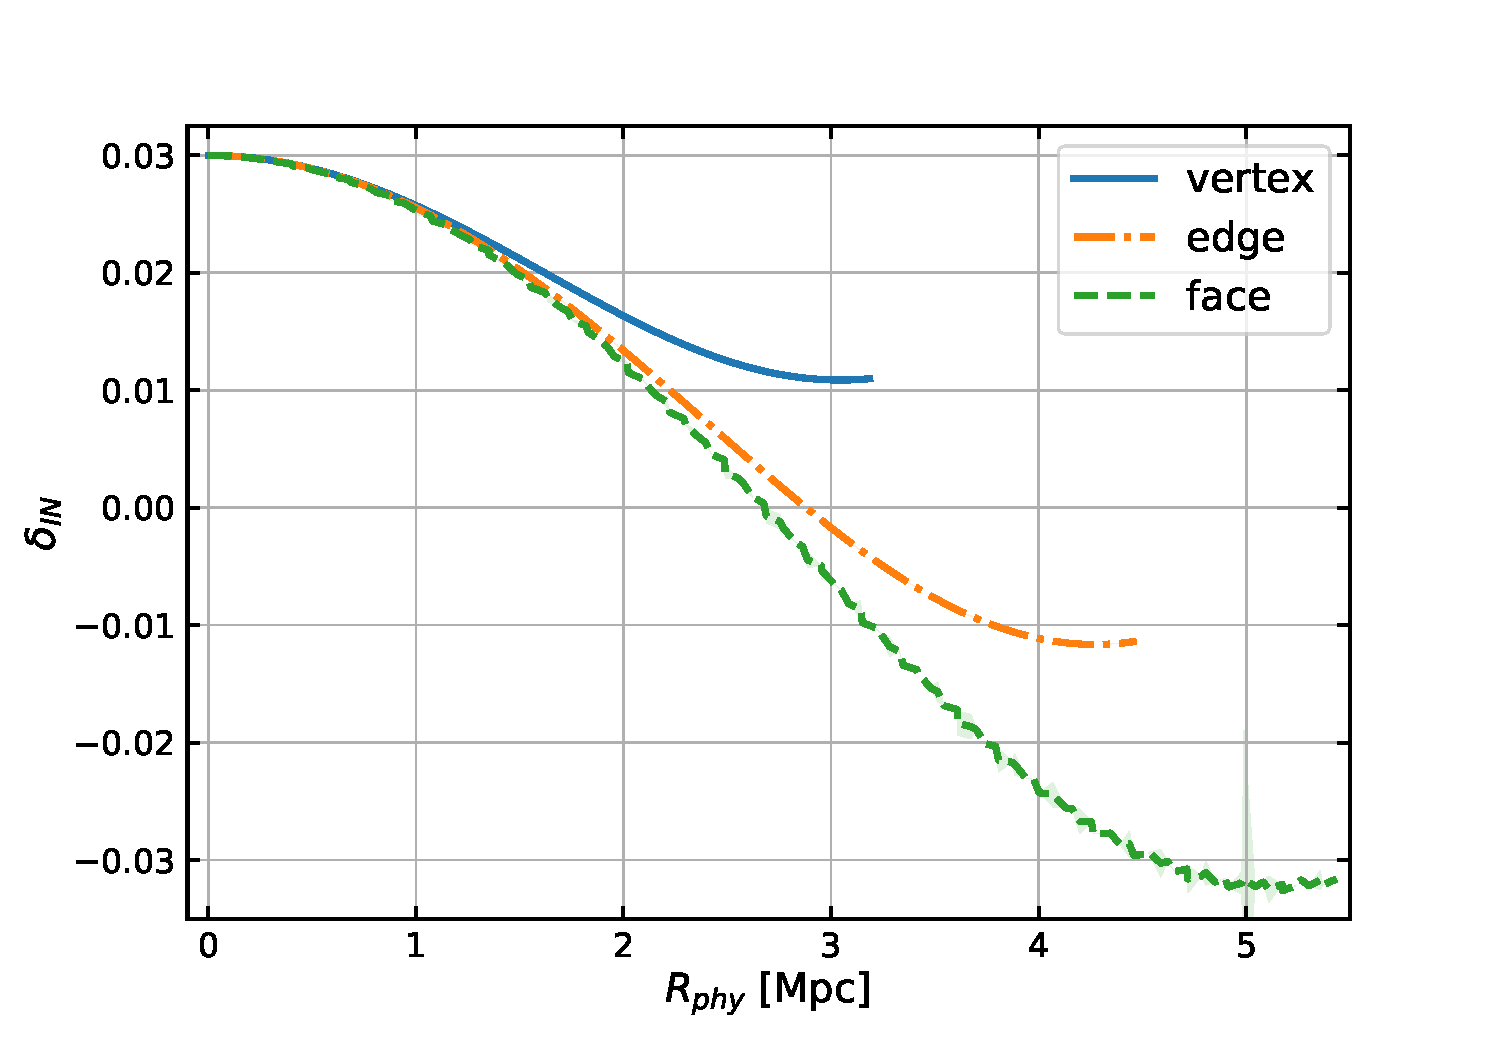
\includegraphics[width=\linewidth]{plots/Paper2/Initial_1d_delta.pdf}
        \caption[Radial profile of initial $\delta$]{Initial radial profile at $z_{IN} = 302.5$ of the initial density contrast $\delta$ starting from the centre of the over-density to its minimum in three different directions, towards the vertices, edges, and faces of the octahedral distribution in \Eqref{eq: Rc} plotted against the proper radius from the over-dense peak. Error bars, when visible, are indicated as shaded regions.}
        \label{fig: IniDelta1d}
    \end{minipage}
    \vspace{0.2cm}
    \begin{minipage}{\linewidth}
        \centering
        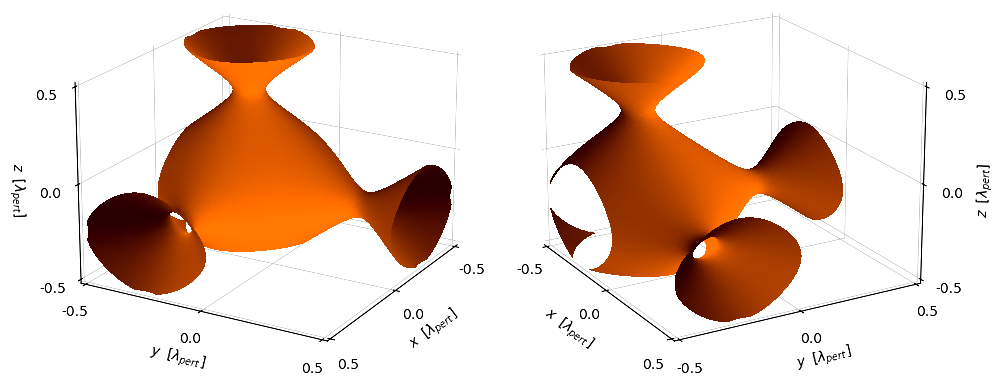
\includegraphics[width=\linewidth]{plots/Paper2/Initial_3d_delta_0d01_isocurve.png}
        \caption[Isosurface of initial $\delta$]{Isosurface for $\delta=0.01$ in the initial distribution of the matter density contrast at $z_{IN} = 302.5$. The two different panels show different points of view. The periodic boundary conditions insure that this distribution is a lattice of over-densities connected by filaments and separated by voids.}
        \label{fig: Isocurve}
    \end{minipage}
\end{figure}

\section{Simulation results} \label{sec: Sim: Results}

\section{Summary} \label{sec: Sim: Conclusion}
